\chapter{Implementacja}

Po zrozumieniu istoty algorytmów rojowych przyszedł czas na zastosowanie tej wiedzy w praktyce. W tym rozdziale zostanie zaprezentowane w jaki sposób jest przedstawiona funkcja obliczająca własności dyspersyjne zwierciadła, jak została na jej podstawie zbudowana funkcja celu oraz jakie zostały zastosowane biblioteki i techniki programistyczne w opracowaniu tego algorytmu.

\section{Metoda macierzy przejścia} \label{macierz} %3.	Opis metody macierzy przejścia 

Pierwszym etapem jest wyznaczenie funkcji pozwalającej na określenie wartości współczynnika odbicia R jak i GDD dla dowolnego zwierciadła DBR. Posłużymy się metodą macierzy przejścia, która polega na wyznaczeniu macierzy przejścia wektora natężenia pola elektrycznego z jednej warstwy do drugiej, a następnie, na tej podstawie, macierzy przejścia dla całej struktury.

Wiązka światłą padająca na zwierciadło DBR jest, zgodnie z istotą korpuskularno-falową światła, falą elektromagnetyczną. Pole elektryczne w każdej z warstw zwierciadła DBR ma postać:
\begin{equation}
    E_m(z) = F_me^{-in_m \frac\omega c z} + B_me^{in_m \frac\omega c z},
\end{equation}

gdzie $F_m$ i $B_m$ odpowiadają fali poruszającej się w kierunku $z$ z kolejno zwrotem dodatnim i ujemnym. \\
Pochodna powyższej wartości ma postać: 

\begin{equation}
    \frac{\partial E_m}{\partial z} = -i n_m \frac\omega c(F_me^{-in_m \frac\omega cz} - B_me^{in_m \frac\omega cz}).
\end{equation}

Na rysunku \ref{fig:transmatr} przedstawiono schemat ilustrujący rozkład sił pola elektrycznego w zwierciadle. Przyjmijmy $F'_m = F_m e^{-i\phi_m}$ i $B'_m = B_m e^{i\phi_m}$, gdzie $\phi = n_m \frac\omega c d_m$.
\begin{figure}[H]
    \centering
    \begin{tikzpicture}
        \draw (3,5) -- (3,0) 
        (1.5,5.3) node {$n_0$}
        (4,5.3) node {$n_1$}
        (3,-0.3) node {$z_0$};
        \draw (5,5) -- (5,0) 
        (6.5,5.3) node {$n_2$}
        (5,-0.3) node {$z_1$};
        \draw (8,5) -- (8,0) 
        (9,5.3) node {$n_3$}
        (8,-0.3) node {$z_2$};
        \draw (10,5) -- (10,0)
        (11.5,2.5) node {...}
        (10,-0.3) node {$z_3$};
        \draw (13,5) -- (13,0)
        (13,-0.3) node {$z_N$}
        (14,5.3) node {$n_N$};
        %skladowe F
        \draw[->] (2.25,3.5) -- (3,3.5) node[above left] {$F_0$};
        \draw[->] (3,3.5) -- (3.75,3.5) node[above] {$F_1$};
        \draw[color = red, ->] (4.25,3.5) -- (5,3.5) node[above left] {$F'_1$};
        \draw[->] (5,3.5) -- (5.75,3.5) node[above] {$F_2$};
        \draw[color = red, ->] (7.25,3.5) -- (8,3.5) node[above left] {$F'_2$};
        \draw[->] (8,3.5) -- (8.75,3.5) node[above] {$F_3$};
        \draw[color = red, ->] (9.25,3.5) -- (10,3.5) node[above left] {$F'_3$};
        \draw[->] (10,3.5) -- (10.75,3.5) node[above] {$F_4$};
        \draw[color = red, ->] (12.25,3.5) -- (13,3.5) node[above left] {$F'_{N-1}$};
        \draw[->] (13,3.5) -- (13.75,3.5) node[above] {$F_N$};
        %skladowe B
        \draw[<-] (2.25,1.5) -- (3,1.5) node[above left] {$B_0$};
        \draw[<-] (3,1.5) -- (3.75,1.5) node[above] {$B_1$};
        \draw[color = red, <-] (4.25,1.5) -- (5,1.5) node[above left] {$B'_1$};
        \draw[<-] (5,1.5) -- (5.75,1.5) node[above] {$B_2$};
        \draw[color = red, <-] (7.25,1.5) -- (8,1.5) node[above left] {$B'_2$};
        \draw[<-] (8,1.5) -- (8.75,1.5) node[above] {$B_3$};
        \draw[color = red, <-] (9.25,1.5) -- (10,1.5) node[above left] {$B'_3$};
        \draw[<-] (10,1.5) -- (10.75,1.5) node[above] {$B_4$};
        \draw[color = red, <-] (12.25,1.5) -- (13,1.5) node[above left] {$B'_{N-1}$};
        \draw[<-] (13,1.5) -- (13.75,1.5) node[above] {$B_{N}$};
    \end{tikzpicture}
    \caption{Schemat zwierciadła DBR}
    \label{fig:transmatr}
\end{figure}

Warunek ciągłości dla poszczególnych warstw można zapisać następująco:
\begin{equation}
    \left\{
    \begin{array}{l}
        F'_m + B'_m = F_{m+1} + B_{m+1}, \\
        n_m(F'_m - B'_m) = n_{m+1}(F_{m+1} - B_{m+1}).
    \end{array}
    \right.
\end{equation}
Rozwiązując powyższy układ równań względem $F'_m$ i $B'_m$ otrzymujemy:

\begin{equation}
    \left[
    \begin{array}{c}
    F_{m+1} \\ B_{m+1}
    \end{array}
    \right] = \frac 12
    \left[
    \begin{array}{cc}
         (1 + \frac{n_m}{n_{m+1}}) &  (1 - \frac{n_m}{n_{m+1}})\\
         (1 - \frac{n_m}{n_{m+1}}) &  (1 + \frac{n_m}{n_{m+1}})
    \end{array}
    \right]
    \left[
    \begin{array}{c}
    F'_{m} \\ B'_{m}
    \end{array}
    \right].
\end{equation}
Korzystając z definicji $F'_m$ i $B'_m$ możemy zapisać:
\begin{equation}
    \left[
    \begin{array}{c}
    F_{m+1} \\ B_{m+1}
    \end{array}
    \right] = \frac 12
    \left[
    \begin{array}{cc}
         (1 + \frac{n_m}{n_{m+1}}) &  (1 - \frac{n_m}{n_{m+1}})\\
         (1 - \frac{n_m}{n_{m+1}}) &  (1 + \frac{n_m}{n_{m+1}})
    \end{array}
    \right]
    \left[
    \begin{array}{c}
    e^{-i\phi_m} \\ e^{i\phi_m}
    \end{array}
    \right]
    \left[
    \begin{array}{c}
    F_{m} \\ B_{m}
    \end{array}
    \right],
\end{equation}
co ostatecznie daje:
\begin{equation}
    \left[
    \begin{array}{c}
    F_{m+1} \\ B_{m+1}
    \end{array}
    \right] = \frac 12
    \left[
    \begin{array}{cc}
         (1 + \frac{n_m}{n_{m+1}})e^{-i\phi_m} &  (1 - \frac{n_m}{n_{m+1}})e^{i\phi_m}\\
         (1 - \frac{n_m}{n_{m+1}})e^{-i\phi_m} &  (1 + \frac{n_m}{n_{m+1}})e^{i\phi_m}
    \end{array}
    \right]
    \left[
    \begin{array}{c}
    F_{m} \\ B_{m}
    \end{array}
    \right].
\end{equation}
Macierz $    \left[
    \begin{array}{cc}
         (1 + \frac{n_m}{n_{m+1}})e^{-i\phi_m} &  (1 - \frac{n_m}{n_{m+1}})e^{i\phi_m}\\
         (1 - \frac{n_m}{n_{m+1}})e^{-i\phi_m} &  (1 + \frac{n_m}{n_{m+1}})e^{i\phi_m}
    \end{array}
    \right]$ nazywamy macierzą przejścia i notujemy $T_m$.
    
Dla lepszej czytelności zapiszmy $E_m =     \left[
    \begin{array}{c}
    F_{m} \\ B_{m}
    \end{array}
    \right]$.
Można zauważyć, że wartość natężenia pola elektrycznego dla danej warstwy zależy od wartości natężenia dla warstwy poprzedniej:
    
\begin{align*}
    &E_1 = T_0 E_0, \\
    &E_2 = T_1 T_0 E_0, \\
    &... \\
    &E_N = (T_N ... T_1 T_0) E_0.
\end{align*}

Iloczyn poszczególnych macierzy przejścia, tj. macierz $T = T_N ... T_1 T_0$, nazywamy macierzą przejścia całej struktury.
Zapiszmy macierz przejścia całej struktury w sposób następujący:
$T = \left[
\begin{array}{cc}
   t_1  & t_2 \\
   t_3  & t_4
\end{array}
\right]$.

Korzystając z tak obliczonej macierzy przejścia można obliczyć amplitudowy współczynnik odbicia, który definiuje stosunek amplitudy fali odbitej do fali padającej. Jako, że $t_3$ odpowiada fali odbitej, natomiast $t_4$ fali padającej, można otrzymać wzór $r=-\frac{t_3}{t_4}$,
%Amplitudowy współczynnik transmisji $t = t_1 - \frac{t_2t_3}{t_4}$
oraz, na tej podstawie, współczynnik odbicia $R = rr^*$.
%Współczynnik transmisji $T = \frac{n_N}{n_0}tt^*$

Grupowe opóźnienie GD (Group Delay) można zdefiniować jako pierwsza pochodna zmiany fazy $\phi$ po częstotliwości $\omega$. Wiemy, że zmianę fazy można zapisać w postaci:
\begin{equation}
    \phi = \arctan\left(\frac{\mathrm{Im}(r)}{\mathrm{Re}(r)}\right),
\end{equation}
stąd GD obliczamy korzystając ze wzoru:

\begin{equation}
    GD = \frac{d\phi}{d\omega} = \frac{\mathrm{Im}(r) \frac{d}{d\omega}\mathrm{Re}(r) - \mathrm{Re}(r) \frac{d}{d\omega}\mathrm{Im}(r)}{rr^*} ,
\end{equation}
natomiast GDD jest pochodną GD po częstotliwości $\omega$, tak jak to przedstawiono we wzorze poniżej:

\begin{equation}
    GDD = \frac{d}{d\omega} GD.
\end{equation}

Tak otrzymane wzory posłużyły do sporządzenia modelu zwierciadła DBR (w postaci klasy) umożliwiającego obliczenie GDD i R dla danego zwierciadła. %Aby dokonać obliczeń wystarczy stworzyć nowy obiekt klasy \textit{DBRMirror} podając dane w postaci współczynników załamania i grubości dla poszczególnych warstw zwierciadła. Stworzenie takiego obiektu skutkuje automatycznym dokonaniem obliczeń i od tego momentu wartości GDD i R są dostępne jako atrybuty tej klasy.

\section{Funkcja celu} \label{sect:cel}

Mając już do dyspozycji wartości GDD i R, należy być w stanie je ocenić przy pomocy funkcji celu, która zostanie użyta w algorytmie rojowym. Celem pracy jest osiągnięcie wartości współczynnika odbicia jak najbliższej jedności, oraz możliwie najmniejszej wartości GDD przy zachowaniu minimalnej zmiany tej wartości w zadanym zakresie długości fali. Dlatego funkcja celu powinna brać pod uwagę następujące aspekty:
\begin{enumerate}
    \item czy wartość R jest bliska jedności poprzez zliczenie ilości wystąpień wartości większych niż $0,98$ na danym przedziale długości fali,
    \item średnia wartości GDD,
    \item wahanie wartości GDD poprzez obliczenie odchylenia standardowego od średniej oraz różnicy między największą i najmniejszą wartością jaką przyjmuje GDD w zadanym przedziale,
\end{enumerate}
warunki te pokazano na rysunku \ref{fig:idealne}. 

\begin{figure}
    \centering
    \begin{tikzpicture}
    \draw[->, thick] (0,0) -- (0,4) node[above]{$R$};
    \draw[->, thick] (0,0) -- (5,0) node[right]{$\lambda$};
    \draw[color=blue] (0.2,0) -- (0.2,3.5) -- (4.8,3.5) -- (4.8,0);
    \node at (2.5,2.3)  {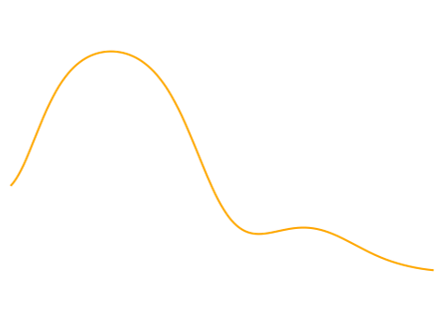
\includegraphics[width=4.8cm]{figures/funkcjacelu/R.png}};
    \draw[thick] (-0.1,3.5) node[left]{1} -- (0.1, 3.5) ;
    \draw[thick, dashed, red] (-0.1,3) node[left]{$0,98$} -- (5,3);
    \draw[->, thick] (9,0) -- (9,4) node[above]{$GDD$};
    \draw[->, thick] (9,3.5) -- (14,3.5) node[right]{$\lambda$};
    \draw[thick] (8.9,0.2) node[left, text width=2cm]{najmniejsza możliwa wartość} -- (9.1, 0.2) ;
    \draw[color=blue] (9.2,3) -- (10.2,3) -- (10.2,0.2) -- (12.8,0.2) -- (12.8,3) -- (13.8,3); 
    \node at (11.5,1.85)  {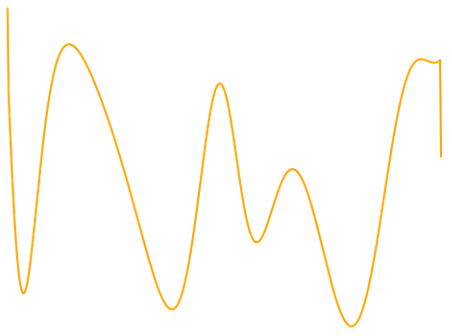
\includegraphics[width=4.8cm]{figures/funkcjacelu/gdd.png}};
    \draw[thick, dashed, red] (8.9,1.6) node[left]{średnia} -- (14,1.6);
    \draw[<->, thick, black!40!green] (11.45,2.75) -- (11.45,1.6);
    \draw[<->, thick, black!40!green] (9.85,3.18) -- (9.85,1.6);
    \draw[<->, thick, black!40!green] (10.93,0.35) -- (10.93,1.6);
   \draw[<->, thick, black!40!green] (11.83,1.06) -- (11.83,1.6);
    \end{tikzpicture}
    \caption{Warunki w funkcji celu}
    Legenda: niebieska krzywa --- funkcja oczekiwana, pomarańczowa krzywa --- funkcja rzeczywista, zielone strzałki --- odchylenie punktu od wartości średniej.
    \label{fig:idealne}
\end{figure}

Do każdego tak ustalonego parametru jest przypisywana waga, która określa w jakim stopniu dany parametr wpływa na wynik końcowy. Im dany parametr jest bliżej żądanej wartości tym bardziej funkcja celu nagradza aktualne rozwiązanie. Otrzymujemy więc 4 wagi, kolejno: $c_R$, $c_{avGDD}$, $c_{devGDD}$, $c_{ptpGDD}$.

W celu sprawdzenia poprawności tak zdefiniowanej funkcji celu, wzięto pod uwagę dwie struktury z wyraźnie różniącym się R i GDD. Dyspersyjne własności pierwszej struktury (pochodzącej z \cite{dbr1}) przedstawiono na rysunku \ref{fig:dbr1}, natomiast drugiej (pochodzącej z \cite{dbr2}) na \ref{fig:dbr2}. Można łatwo zauważyć, że w przypadku obu struktur odbijalność jest na prawidłowym poziomie, natomiast GDD w przypadku struktury 1 charakteryzuje się wyraźnym pikiem w granicach $1055\nm$. Struktura 2 natomiast charakteryzuje się GDD prawie, że stałym na poziomie $800\,\mathrm{fs^2}$. Z pełną pewnością można stwierdzić, że struktura 2 jest lepsza od struktury 1.

\begin{figure}
    \centering
    \begin{subfigure}[b]{0.46\textwidth}
        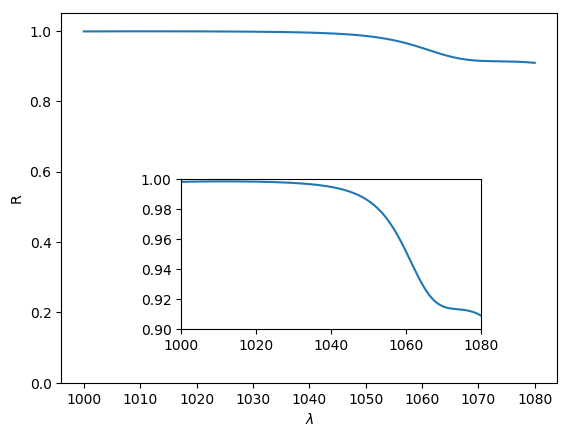
\includegraphics[width=\linewidth]{figures/funkcjacelu/result_Rdbr.png}
        \caption{R (przedstawione również w powiększeniu)}
    \end{subfigure}
       \begin{subfigure}[b]{0.49\textwidth}
        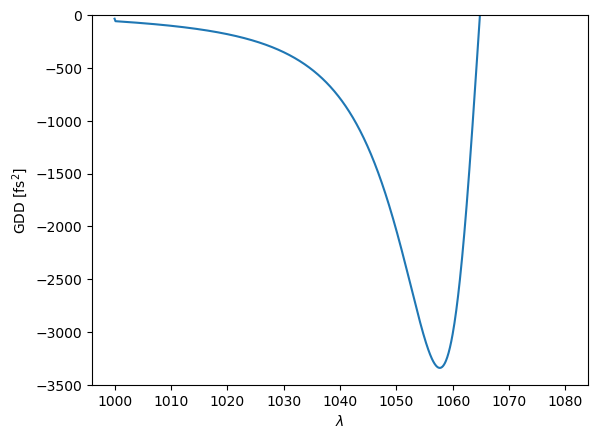
\includegraphics[width=\linewidth]{figures/funkcjacelu/result_gdddbr.png}
        \caption{GDD\\~}
    \end{subfigure}
    \caption[Dyspersyjne własności struktury 1 (gorszej)]{Dyspersyjne własności struktury 1 z \cite{dbr1} (gorszej)}
    \label{fig:dbr1}
\end{figure}

\begin{figure}
    \centering
    \begin{subfigure}[b]{0.46\textwidth}
        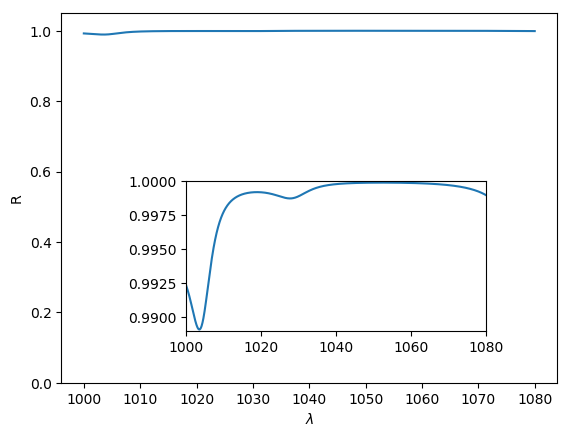
\includegraphics[width=\linewidth]{figures/funkcjacelu/result_Rdbr_opt.png}
        \caption{R (przedstawione również w powiększeniu)}
    \end{subfigure}
       \begin{subfigure}[b]{0.49\textwidth}
        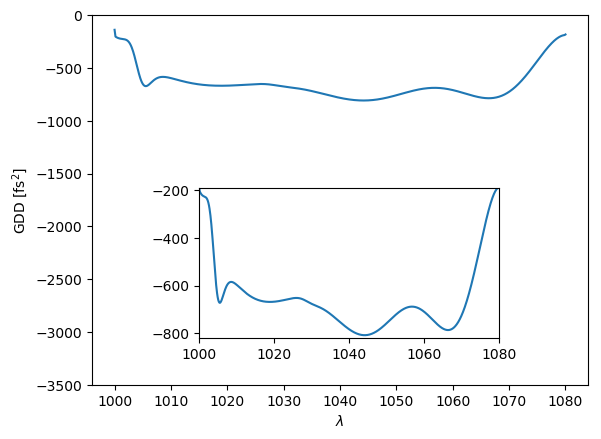
\includegraphics[width=\linewidth]{figures/funkcjacelu/result_gdddbr_opt.png}
        \caption{GDD (przedstawione również w powiększeniu)}
    \end{subfigure}
    \caption[Dyspersyjne własności struktury 2 (lepszej)]{Dyspersyjne własności struktury 2 z \cite{dbr2} (lepszej)}
    \label{fig:dbr2}
\end{figure}

Wykonano obliczenia dla dwóch różnych wartości wag i otrzymano wyniki przedstawione w tabeli \ref{tab:funkcel}.

\begin{table}[H]
    \centering
    \caption{Weryfikacja działania funkcji celu}
    \begin{tabular}{|c|c|c|c|c|c|} \cline{5-6}
        \multicolumn{4}{c}{} & \multicolumn{2}{|c|}{Wartość funkcji celu} \\\hline
         $c_R$ & $c_{avGDD}$& $c_{devGDD}$& $c_{ptpGDD}$ &  Struktura 1 (gorsza) & Struktura 2 (lepsza)\\\hline
         $0,5$ &$2$ &$10$& $1$& $69,596$ &$459,668$ \\\hline
         $100000$ & $70$& $1$& $0$& $4583.742$ & $50419.277$ \\\hline
    \end{tabular}
    \label{tab:funkcel}
\end{table}

Obserwując wyniki z tabeli \ref{tab:funkcel} widać wyraźnie, że struktura 2 dostała znacznie lepszą ocenę niż struktura 1, która została uznana za gorszą na podstawie obserwacji wykresów z rysunków \ref{fig:dbr1} i \ref{fig:dbr2}. Więc funkcja celu działa w sposób prawidłowy i można jej użyć w algorytmie rojowym. 

\section{Przedstawienie danych wejściowych i wyniki}
W celu uproszczenia problemu, założono, że zwierciadło jest zbudowane ze stałej liczby naprzemiennych warstw dwóch materiałów półprzewodnikowych: arsenku glinu AlAs oraz arsenku galu GaAs o współczynnikach załamania światła kolejno $n_1=2,956$ i $n_2=3,489$, które są również stałe podczas działania algorytmu. Dlatego też wystarczające będzie przedstawienie danych wejściowych w postaci grubości warstw do zastosowania algorytmu rojowego. Wprowadza to dużą losowość uzyskanych wyników, dlatego wykonano również obliczenia przedstawiając dane w postaci zmiennej wynikającej z warunku Bragg'a. Ponadto, sprawdzono wpływ przedstawienia danych w postaci dwóch parametrów: zmiennej wynikającej z warunku Bragg'a oraz zależności między grubościami warstw w parze. W dalszej części tekstu zostały przedstawione dokładne zależności między warstwami jakie zostały wzięte pod uwagę oraz wyniki jakie uzyskano dla każdego omawianego przypadku.

\subsection{Losowanie grubości warstw}

W pierwszej kolejności zastosowano bezpośrednio grubości warstw struktury złożonej ze 122 powłok kolejno GaAs i AlAs. Pierwsze $N$ rozwiązań jest generowane losowo w przedziale $\langle 5\nm, 1000\nm \rangle$. Otrzymane tak wyniki przedstawiono na rysunku \ref{fig:wynlosd}.

\begin{figure} [H]
    \centering
    \begin{subfigure}[b]{0.30\textwidth}
        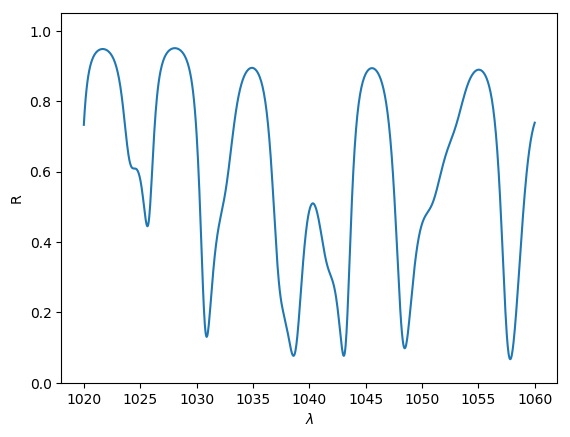
\includegraphics[width=\linewidth]{figures/wyniki/losowe/d/result_Rresult0.png}
        \caption{R w iteracji 0}
    \end{subfigure}
            \begin{subfigure}[b]{0.31\textwidth}
        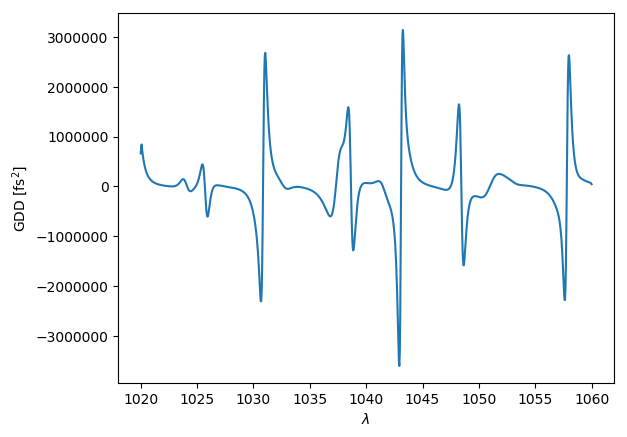
\includegraphics[width=\linewidth]{figures/wyniki/losowe/d/result_gddresult0.png}
        \caption{GDD w iteracji 0}
    \end{subfigure}
            \begin{subfigure}[b]{0.32\textwidth}
        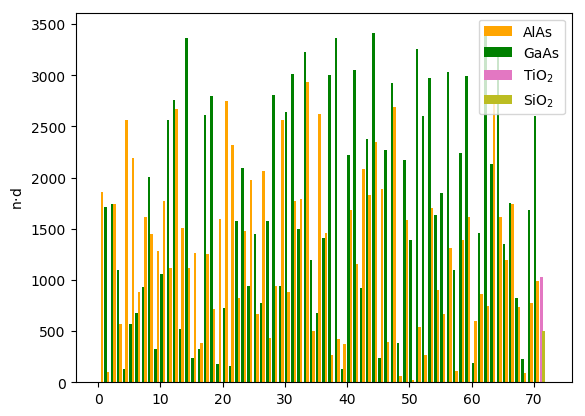
\includegraphics[width=\linewidth]{figures/wyniki/losowe/d/result_ndresult0.png}
        \caption{Iloczyn $nd$ w iteracji 0}
    \end{subfigure}
        \begin{subfigure}[b]{0.30\textwidth}
        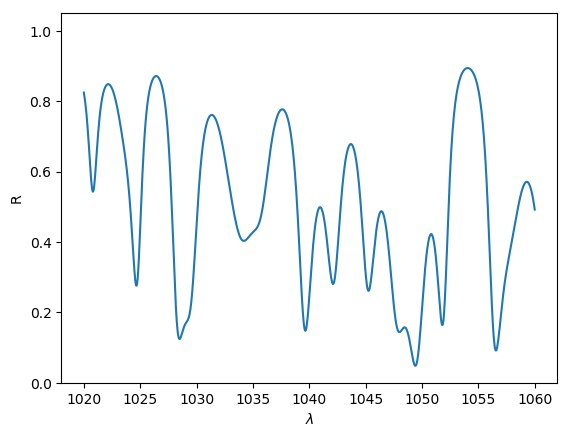
\includegraphics[width=\linewidth]{figures/wyniki/losowe/d/result_Rresult499.png}
        \caption{R w iteracji 499}
    \end{subfigure}
        \begin{subfigure}[b]{0.31\textwidth}
        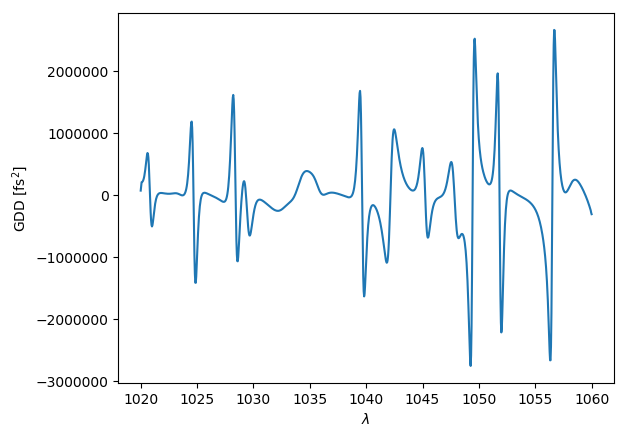
\includegraphics[width=\linewidth]{figures/wyniki/losowe/d/result_gddresult499.png}
        \caption{GDD w iteracji 499}
    \end{subfigure}
        \begin{subfigure}[b]{0.32\textwidth}
        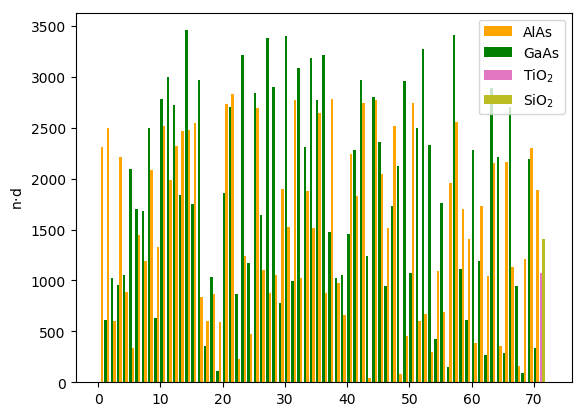
\includegraphics[width=\linewidth]{figures/wyniki/losowe/d/result_ndresult499.png}
        \caption{Iloczyn $nd$ w iteracji 499}
    \end{subfigure}
    \caption{Wyniki obliczeń w przypadku losowania grubości warstw przy rozpoczęciu obliczeń od losowo wygenerowanej struktury}
    Wartości parametrów: $N=1000$, $d_{near}= 0,005$, $w_{qual}=0,40$, $w_{best}=0,20$, $w_{better}=0,8$, $p_1=0,5$, $p_2=2$, $p_3=10$, $p_4=1$
    \label{fig:wynlosd}
\end{figure}

Można zauważyć, że wyniki wyglądają bardzo źle, ale widać jednocześnie zmianę wynikowej struktury co świadczy o działaniu programu. Można wywnioskować, że rozpoczynając obliczenia w sposób zupełnie losowy jest bardzo mało prawdopodobne znalezienie rozwiązań dobrych. Dlatego postanowiono generować pierwsze $N$ rozwiązań generując rozwiązania z dalekiego sąsiedztwa $d_{far}$ struktury już wcześniej znanej. W tym celu zostały wykorzystane struktury 1 i 2 omawiane w podrozdziale \ref{sect:cel}. Wyniki zostały przedstawione na rysunkach \ref{fig:wynlos1} i \ref{fig:wynlos2}. Parametry zostały dobrane w identyczny sposób jak w przypadku rysunku \ref{fig:wynlosd}, natomiast wartość parametru $d_{far}$ wynosi $50$.

\begin{figure} [H]
    \centering
    \begin{subfigure}[b]{0.30\textwidth}
        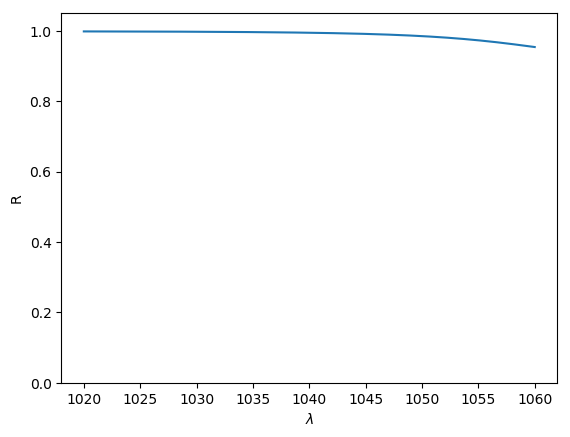
\includegraphics[width=\linewidth]{figures/wyniki/losowe/dbr/result_Rresult0.png}
        \caption{R w iteracji 0}
    \end{subfigure}
            \begin{subfigure}[b]{0.31\textwidth}
        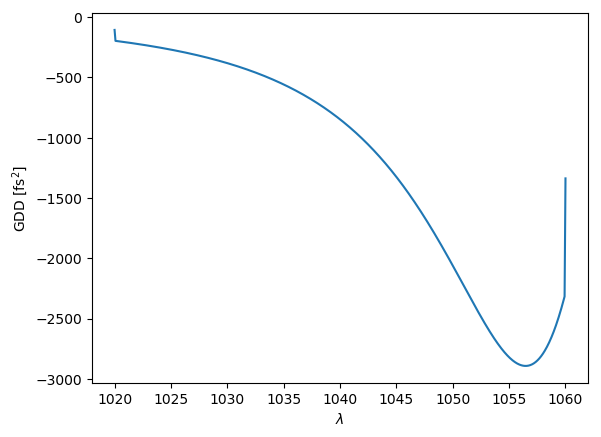
\includegraphics[width=\linewidth]{figures/wyniki/losowe/dbr/result_gddresult0.png}
        \caption{GDD w iteracji 0}
    \end{subfigure}
            \begin{subfigure}[b]{0.32\textwidth}
        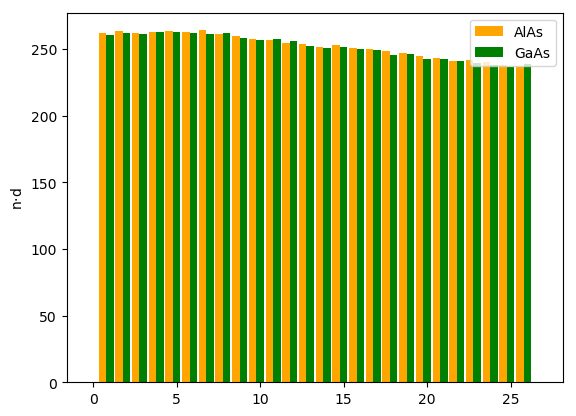
\includegraphics[width=\linewidth]{figures/wyniki/losowe/dbr/result_ndresult0.png}
        \caption{Iloczyn $nd$ w iteracji 0}
    \end{subfigure}
        \begin{subfigure}[b]{0.30\textwidth}
        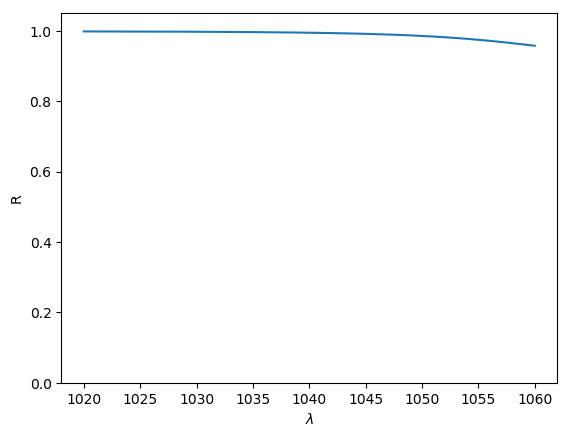
\includegraphics[width=\linewidth]{figures/wyniki/losowe/dbr/result_Rresult499.png}
        \caption{R w iteracji 499}
    \end{subfigure}
        \begin{subfigure}[b]{0.31\textwidth}
        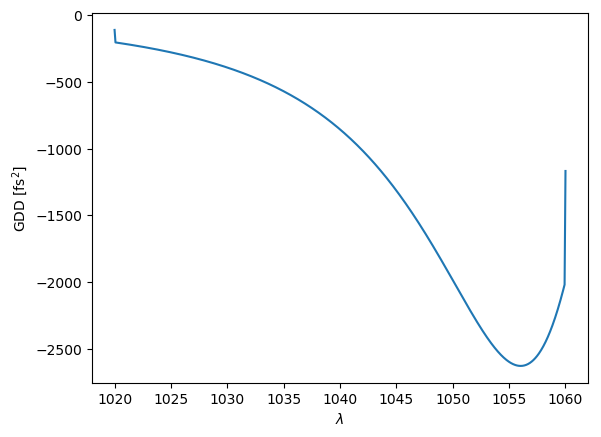
\includegraphics[width=\linewidth]{figures/wyniki/losowe/dbr/result_gddresult499.png}
        \caption{GDD w iteracji 499}
    \end{subfigure}
        \begin{subfigure}[b]{0.32\textwidth}
        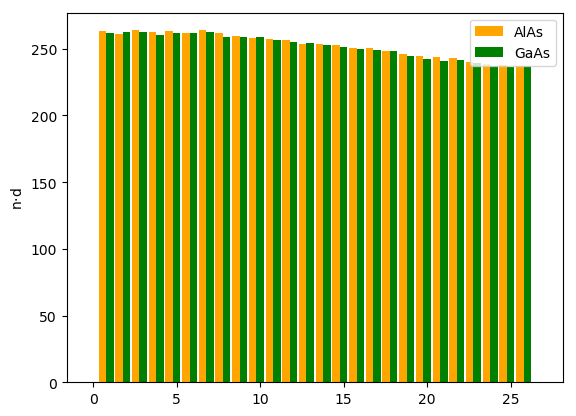
\includegraphics[width=\linewidth]{figures/wyniki/losowe/dbr/result_ndresult499.png}
        \caption{Iloczyn $nd$ w iteracji 499}
    \end{subfigure}
    \caption{Wyniki obliczeń w przypadku losowania grubości warstw przy rozpoczęciu obliczeń od struktury 1 (gorszej)}
    \label{fig:wynlos1}
\end{figure}

\begin{figure} [H]
    \centering
    \begin{subfigure}[b]{0.30\textwidth}
        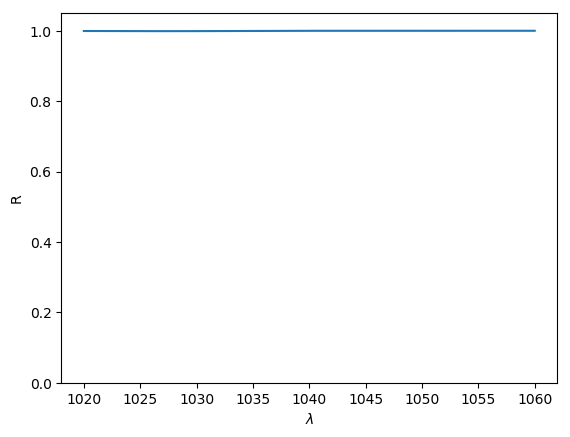
\includegraphics[width=\linewidth]{figures/wyniki/losowe/dbr_opt/result_Rresult0.png}
        \caption{R w iteracji 0}
    \end{subfigure}
            \begin{subfigure}[b]{0.31\textwidth}
        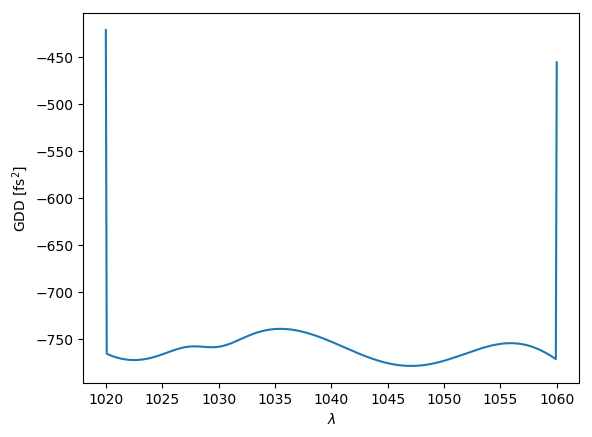
\includegraphics[width=\linewidth]{figures/wyniki/losowe/dbr_opt/result_gddresult0.png}
        \caption{GDD w iteracji 0}
    \end{subfigure}
            \begin{subfigure}[b]{0.32\textwidth}
        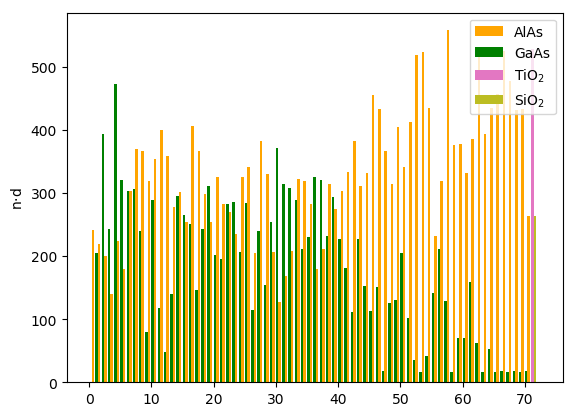
\includegraphics[width=\linewidth]{figures/wyniki/losowe/dbr_opt/result_ndresult0.png}
        \caption{Iloczyn $nd$ w iteracji 0}
    \end{subfigure}
        \begin{subfigure}[b]{0.30\textwidth}
        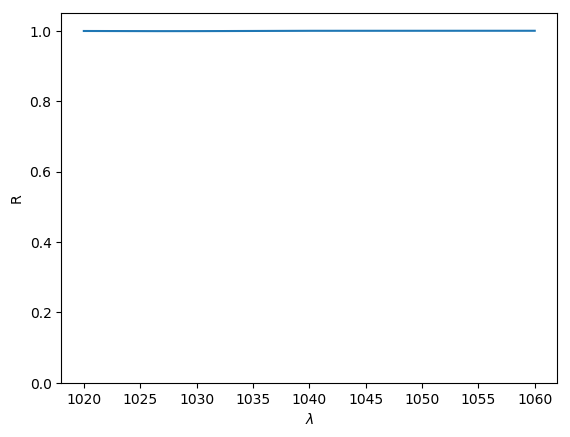
\includegraphics[width=\linewidth]{figures/wyniki/losowe/dbr_opt/result_Rresult499.png}
        \caption{R w iteracji 499}
    \end{subfigure}
        \begin{subfigure}[b]{0.31\textwidth}
        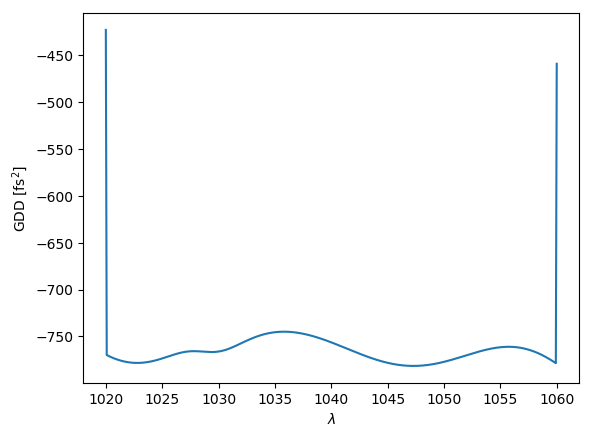
\includegraphics[width=\linewidth]{figures/wyniki/losowe/dbr_opt/result_gddresult499.png}
        \caption{GDD w iteracji 499}
    \end{subfigure}
        \begin{subfigure}[b]{0.32\textwidth}
        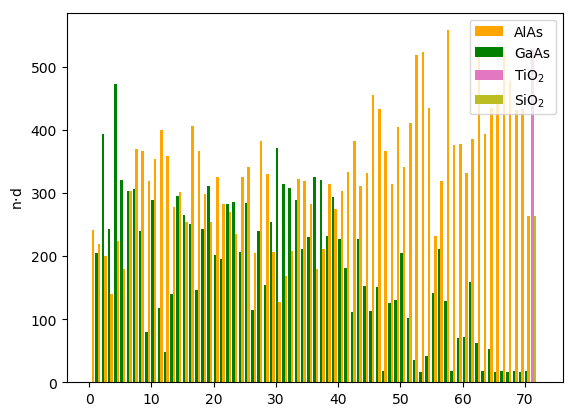
\includegraphics[width=\linewidth]{figures/wyniki/losowe/dbr_opt/result_ndresult499.png}
        \caption{Iloczyn $nd$ w iteracji 499}
    \end{subfigure}
    \caption{Wyniki obliczeń w przypadku losowania grubości warstw przy rozpoczęciu obliczeń od struktury 2 (lepszej)}
    \label{fig:wynlos2}
\end{figure}
\newpage
Można zauważyć, że dla lepszej struktury otrzymano wyniki zdecydowanie lepsze, co dowodzi, że to jest dobry sposób na lekkie polepszenie już istniejącej struktury, jednocześnie nie umożliwiając stworzenia nowej struktury zupełnie od zera. Dodatkowo można zauważyć, że w przypadku \ref{fig:wynlos2} najlepsza struktura nie zmieniła się po 499 iteracjach, co ilustruje trudność otrzymania w ten sposób rozwiązań naprawdę dobrych.

Dodatkowo powtórzono obliczenia z rysunku \ref{fig:wynlos2}, lecz wykorzystując tym razem 100 razy większą ilości pszczół zwiadowców przy mniejszej ilości iteracji (ze względu na ich znaczącą długość). Otrzymane wyniki przedstawiono na rysunku \ref{fig:wynlos3}. Można zauważyć, że różnice między otrzymanymi wykresami nie są znaczące i zmiana tego parametru nie ma wpływu na wynik w tym wypadku.

\begin{figure} [H]
    \centering
    \begin{subfigure}[b]{0.30\textwidth}
        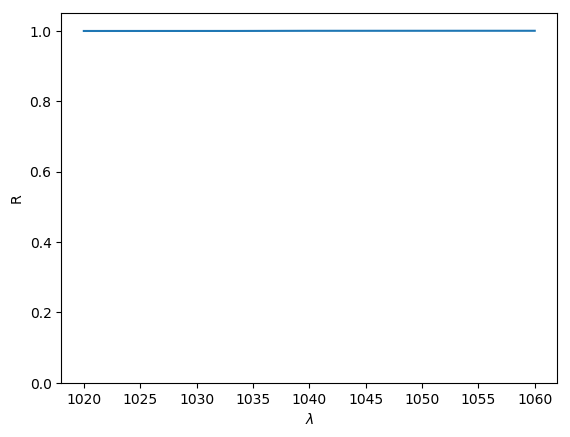
\includegraphics[width=\linewidth]{figures/wyniki/losowe/dbr_opt10/result_Rresult0.png}
        \caption{R w iteracji 0}
    \end{subfigure}
            \begin{subfigure}[b]{0.31\textwidth}
        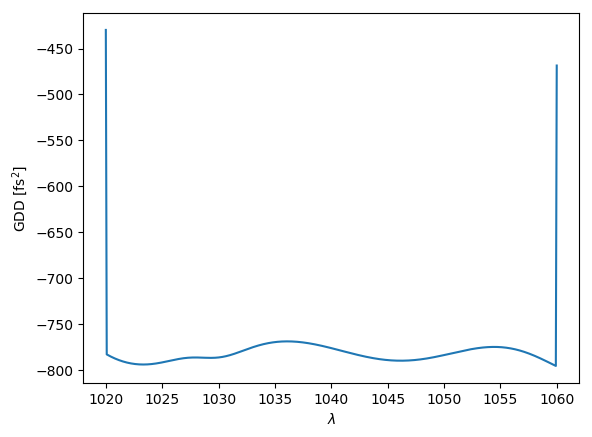
\includegraphics[width=\linewidth]{figures/wyniki/losowe/dbr_opt10/result_gddresult0.png}
        \caption{GDD w iteracji 0}
    \end{subfigure}
            \begin{subfigure}[b]{0.32\textwidth}
        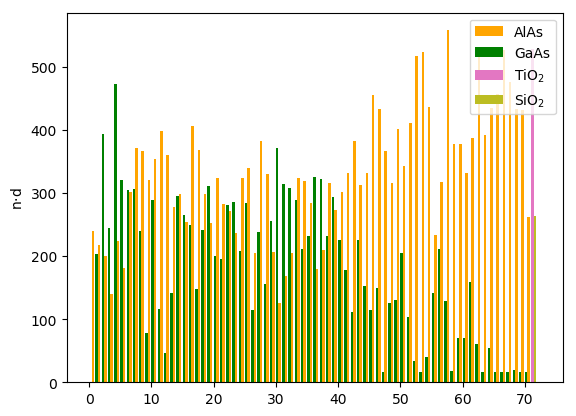
\includegraphics[width=\linewidth]{figures/wyniki/losowe/dbr_opt10/result_ndresult0.png}
        \caption{Iloczyn $nd$ w iteracji 0}
    \end{subfigure}
        \begin{subfigure}[b]{0.30\textwidth}
        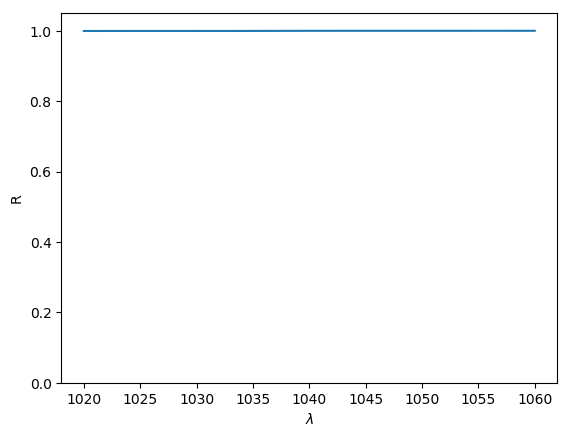
\includegraphics[width=\linewidth]{figures/wyniki/losowe/dbr_opt10/result_Rresult10.png}
        \caption{R w iteracji 10}
    \end{subfigure}
        \begin{subfigure}[b]{0.31\textwidth}
        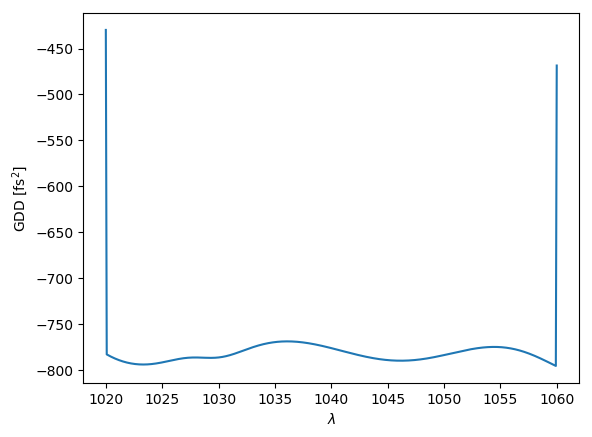
\includegraphics[width=\linewidth]{figures/wyniki/losowe/dbr_opt10/result_gddresult10.png}
        \caption{GDD w iteracji 10}
    \end{subfigure}
        \begin{subfigure}[b]{0.32\textwidth}
        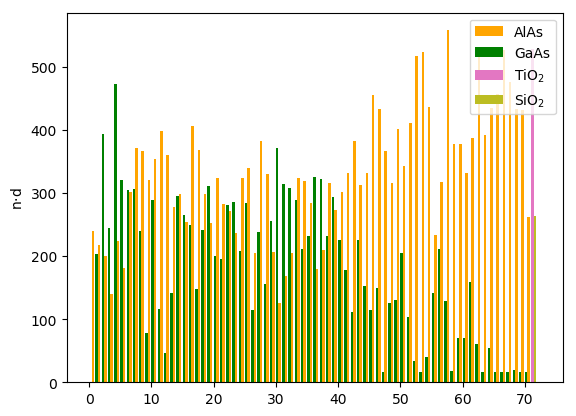
\includegraphics[width=\linewidth]{figures/wyniki/losowe/dbr_opt10/result_ndresult10.png}
        \caption{Iloczyn $nd$ w iteracji 10}
    \end{subfigure}
    \caption{Wyniki obliczeń w przypadku losowania grubości warstw przy rozpoczęciu obliczeń od struktury 2 (lepszej) i $N = 100000$ pszczół}
    \label{fig:wynlos3}
\end{figure}

\subsection{Losowanie parametru wykorzystującego warunek Bragg'a} % df = n_warstw - n_warstw/2
Następnie, aby polepszyć uzyskiwanie wyniki i zminimalizować losowość, skorzystano z warunku Bragg'a:
\begin{equation}
    n_1d_1 + n_2d_2 = \frac{\lambda_B}{2}, \label{eq:bragg}
\end{equation}
gdzie $n_1$, $n_2$ --- współczynniki załamania warstw $1$ i $2$, $d_1$, $d_2$ --- grubości warstw $1$ i $2$, $\lambda_B$ --- długość fali Bragg'a czyli długość fali dla której zwierciadło osiąga maksimum odbijalności. Warunek ten posłużył do wprowadzenia zmiennej $c$, zdefiniowanej według wzoru:
\begin{equation}
    \lambda_B = \lambda c. \label{eq:c}
\end{equation}
Wartość $\lambda$ oznacza środek właśnie badanego przedziału długości fali. Tak dobrana zmienna $c$ oscyluje w przedziale $\langle 0,5, 1,5 \rangle$, a co za tym idzie $\lambda_B$ przyjmuje wartości od $500\nm$ do $1500\nm$ przy $\lambda = 1000\nm$. Dodatkowo wprowadzono warunek na zachowanie równości iloczynu $nd$ dla każdej z warstw w danej parze, zgodnie ze wzorem $n_1d_1=n_2d_2$. Na tej podstawie otrzymano następujące wzory na grubości warstw w parze: 

\begin{equation}
    \left\{ \begin{array}{c}
         d_1 = \frac{c\lambda}{4n_1}, \\ d_2 = \frac{c\lambda}{4n_2},
    \end{array}\right.
\end{equation}
natomiast wartość $c$ można obliczyć podstawiając \ref{eq:c} do \ref{eq:bragg}, co daje następujące równanie:
\begin{equation}
    c = \frac{2}{\lambda} \cdot (n_1d_1 + n_2d_2).
\end{equation}
Tak otrzymane równania posłużyły do stworzenia funkcji konwersji z grubości warstw do zmiennej $c$ i w odwrotnym kierunku. W tym momencie możliwe było już zastosowanie zmiennej $c$ w algorytmie rojowym. Tak też zostało zrobione i po licznym próbach korzystając z różnych wartości wag funkcji celu, udało się uzyskać wyniki przedstawione na rysunku \ref{fig:wyn1stp} korzystając ze współczynników załamania struktury 1 (gorszej). Dodatkowo wykonano dla tych samych parametrów następne obliczenia na rysunku \ref{fig:wyn1stpopt1} tym razem korzystając z zestawu współczynników odbicia ze struktury 2 (lepszej). Na koniec wykonano jeszcze obliczenia zwiększając liczbę pszczół zwiadowców 100 krotnie względem \ref{fig:wyn1stpopt1} i przedstawiono wyniki na rysunku \ref{fig:wyn1stpopt2}.


\begin{figure} [ht!]
    \centering
    \begin{subfigure}[b]{0.30\textwidth}
        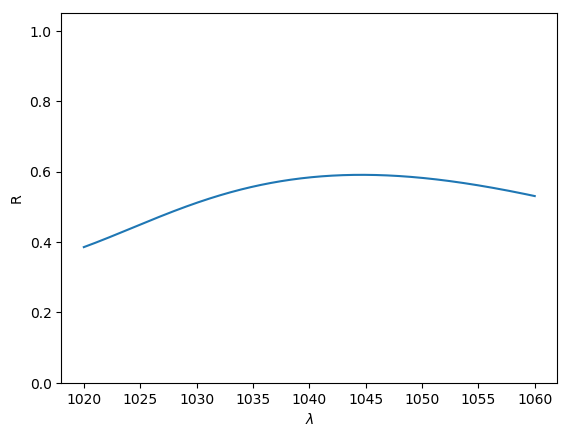
\includegraphics[width=\linewidth]{figures/wyniki/1stopien/fcelptp/result_R0.png}
        \caption{R w iteracji 0}
    \end{subfigure}
            \begin{subfigure}[b]{0.31\textwidth}
        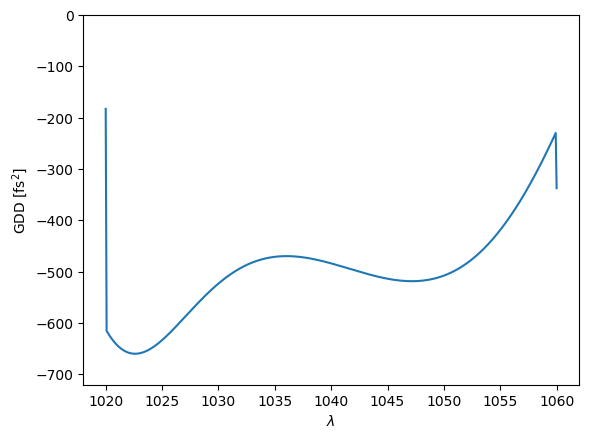
\includegraphics[width=\linewidth]{figures/wyniki/1stopien/fcelptp/result_gdd0.png}
        \caption{GDD w iteracji 0}
    \end{subfigure}
        \begin{subfigure}[b]{0.32\textwidth}
        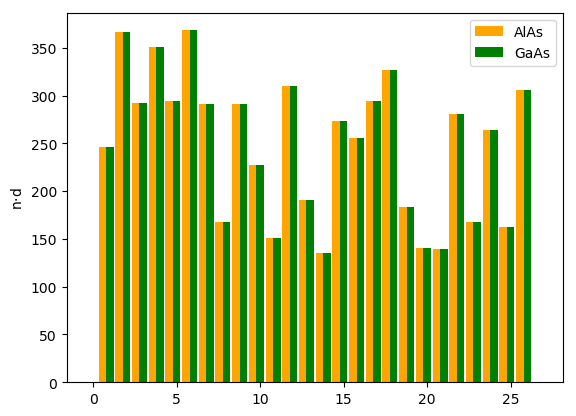
\includegraphics[width=\linewidth]{figures/wyniki/1stopien/fcelptp/result_nd0.png}
        \caption{Iloczyn $nd$ w iteracji 0}
    \end{subfigure}
        \begin{subfigure}[b]{0.30\textwidth}
        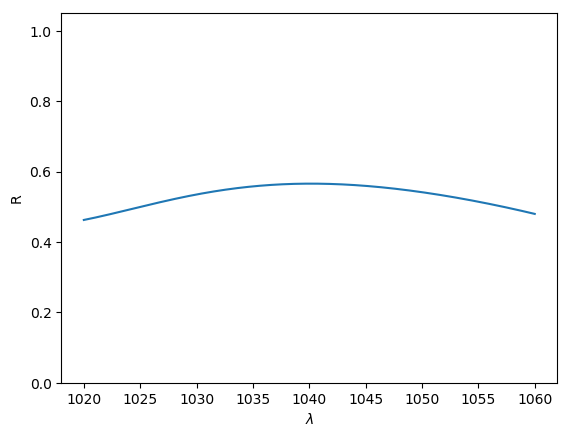
\includegraphics[width=\linewidth]{figures/wyniki/1stopien/fcelptp/result_R1.png}
        \caption{R w iteracji 499}
    \end{subfigure}
        \begin{subfigure}[b]{0.31\textwidth}
        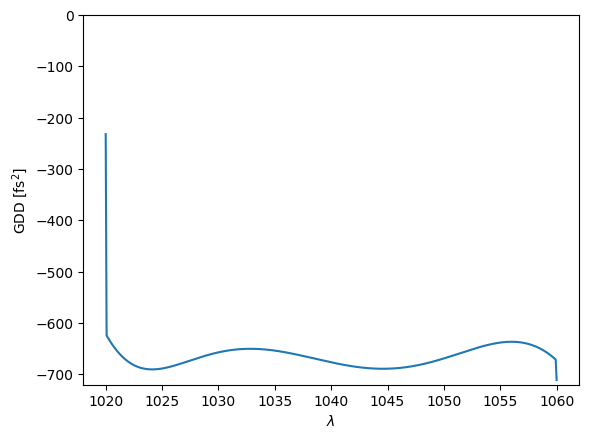
\includegraphics[width=\linewidth]{figures/wyniki/1stopien/fcelptp/result_gdd1.png}
        \caption{GDD w iteracji 499}
    \end{subfigure}
        \begin{subfigure}[b]{0.32\textwidth}
        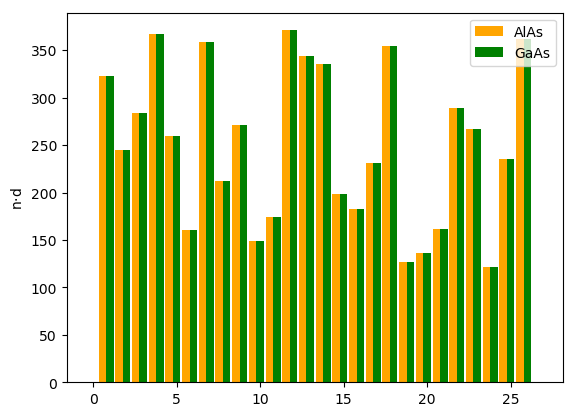
\includegraphics[width=\linewidth]{figures/wyniki/1stopien/fcelptp/result_nd1.png}
        \caption{Iloczyn $nd$ w iteracji 499}
    \end{subfigure}
    \caption{Wyniki obliczeń w przypadku losowania parametru wykorzystującego warunek Bragg'a przy wykorzystaniu współczynników załamania ze struktury 1}
    Wartości parametrów: $N= 1000$, $d_{near}= 0,005$, $w_{qual}=0,40$, $w_{best}=0,20$, $w_{better}=0,8$, $p_1=0,5$, $p_2=2$, $p_3=10$, $p_4=1$
    \label{fig:wyn1stp}
\end{figure}

Można zauważyć na podstawie przedstawionych wyników, że otrzymane wyniki są gorsze od uzyskanego na rysunku \ref{fig:wynlos2}. Dodatkowo iloczyny $nd$ dla każdej warstwy z danej pary są równe, co świadczy o działaniu programu w sposób pożądany. Dodatkowo można zaobserwować ciekawy rezultat --- wyniki korzystające ze struktury teoretycznie gorszej dały zauważalnie lepszy wynik niż te korzystające ze struktury teoretycznie lepszej. Oprócz tego widać, że obliczenia przy większej ilości pszczół zwiadowców (rysunek \ref{fig:wyn1stpopt2} dają gorsze rezultaty niż te przy mniejszej ich ilości (rysunek \ref{fig:wyn1stpopt1}), w odróżnieniu od podejścia korzystającego z samych grubości warstw.

\begin{figure} [H]
    \centering
    \begin{subfigure}[b]{0.30\textwidth}
        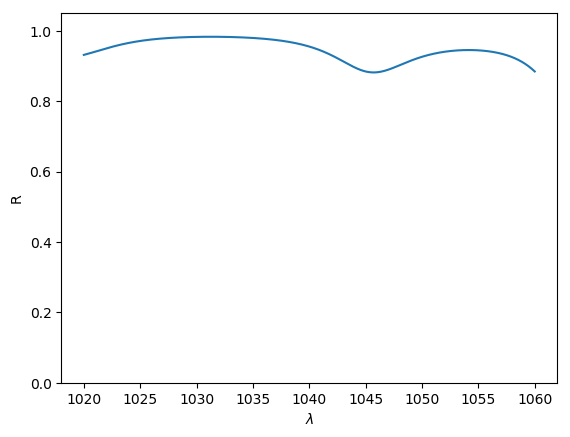
\includegraphics[width=\linewidth]{figures/wyniki/1stopien/opt1000/result_Rresult0.png}
        \caption{R w iteracji 0}
    \end{subfigure}
            \begin{subfigure}[b]{0.31\textwidth}
        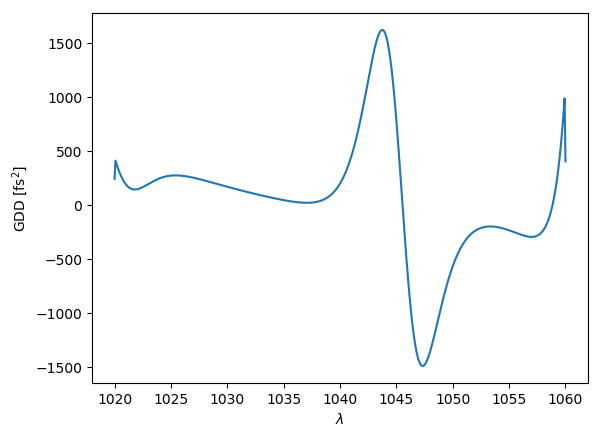
\includegraphics[width=\linewidth]{figures/wyniki/1stopien/opt1000/result_gddresult0.png}
        \caption{GDD w iteracji 0}
    \end{subfigure}
            \begin{subfigure}[b]{0.32\textwidth}
        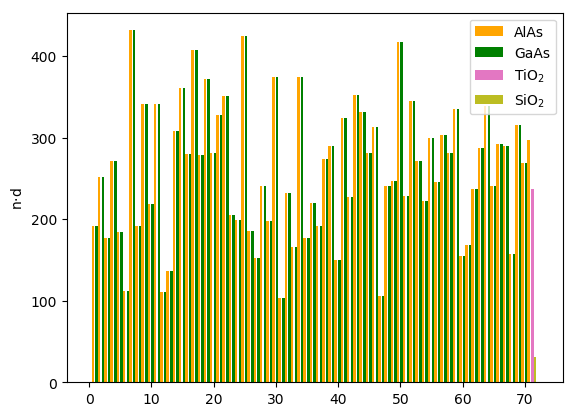
\includegraphics[width=\linewidth]{figures/wyniki/1stopien/opt1000/result_ndresult0.png}
        \caption{Iloczyn $nd$ w iteracji 0}
    \end{subfigure}
        \begin{subfigure}[b]{0.30\textwidth}
        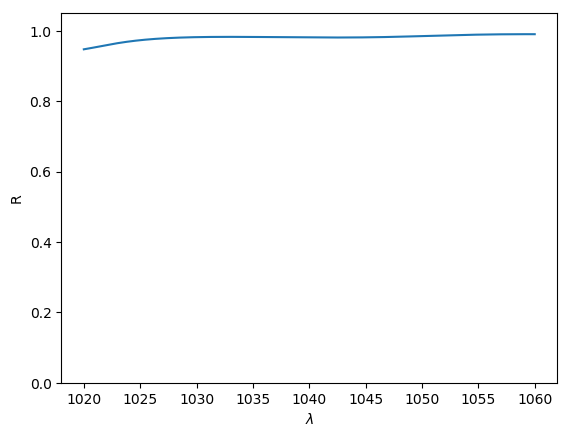
\includegraphics[width=\linewidth]{figures/wyniki/1stopien/opt1000/result_Rresult499.png}
        \caption{R w iteracji 499}
    \end{subfigure}
        \begin{subfigure}[b]{0.31\textwidth}
        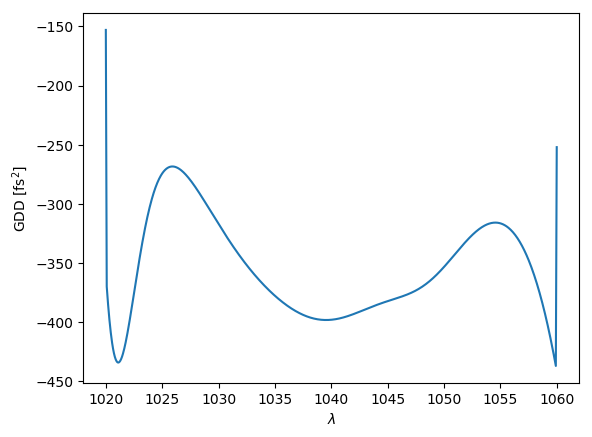
\includegraphics[width=\linewidth]{figures/wyniki/1stopien/opt1000/result_gddresult499.png}
        \caption{GDD w iteracji 499}
    \end{subfigure}
        \begin{subfigure}[b]{0.32\textwidth}
        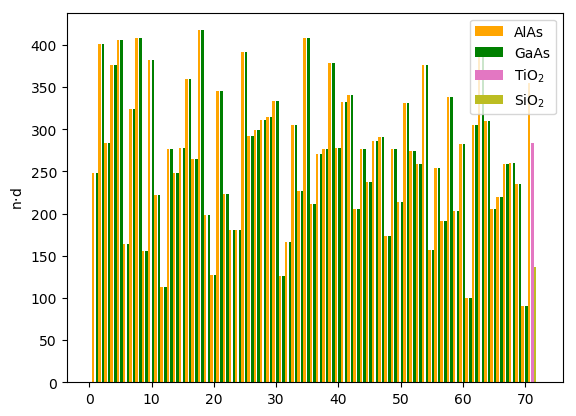
\includegraphics[width=\linewidth]{figures/wyniki/1stopien/opt1000/result_ndresult499.png}
        \caption{Iloczyn $nd$ w iteracji 499}
    \end{subfigure}
    \caption{Wyniki obliczeń w przypadku losowania parametru wykorzystującego warunek Bragg'a przy wykorzystaniu współczynników załamania ze struktury 2}
    Wartości parametrów: $N= 1000$, $d_{near}= 0,005$, $w_{qual}=0,40$, $w_{best}=0,20$, $w_{better}=0,8$, $p_1=0,5$, $p_2=2$, $p_3=10$, $p_4=1$
    \label{fig:wyn1stpopt1}
\end{figure}

\begin{figure} [H]
    \centering
    \begin{subfigure}[b]{0.30\textwidth}
        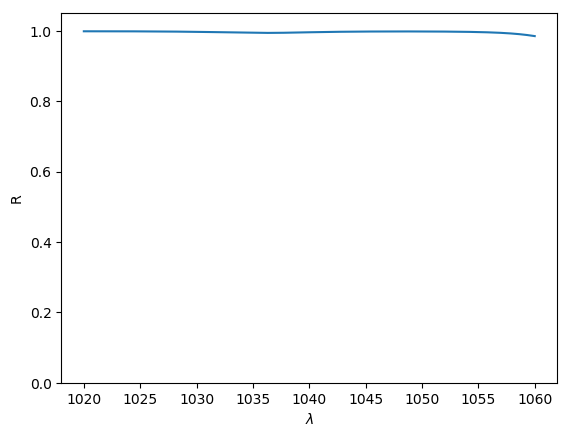
\includegraphics[width=\linewidth]{figures/wyniki/1stopien/opt10^5/result_Rresult0.png}
        \caption{R w iteracji 0}
    \end{subfigure}
            \begin{subfigure}[b]{0.31\textwidth}
        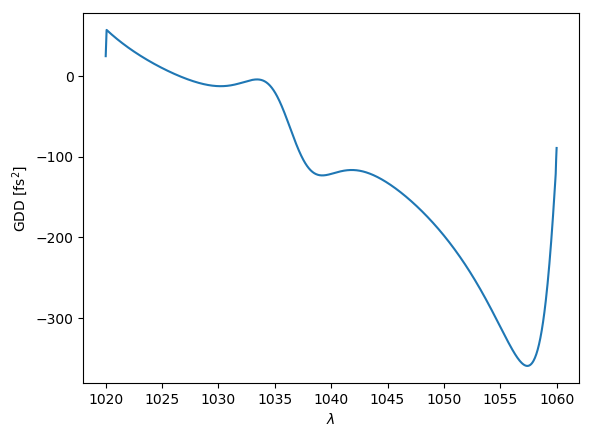
\includegraphics[width=\linewidth]{figures/wyniki/1stopien/opt10^5/result_gddresult0.png}
        \caption{GDD w iteracji 0}
    \end{subfigure}
            \begin{subfigure}[b]{0.32\textwidth}
        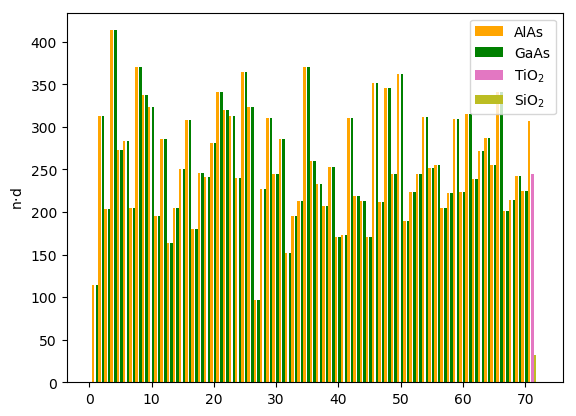
\includegraphics[width=\linewidth]{figures/wyniki/1stopien/opt10^5/result_ndresult0.png}
        \caption{Iloczyn $nd$ w iteracji 0}
    \end{subfigure}
        \begin{subfigure}[b]{0.30\textwidth}
        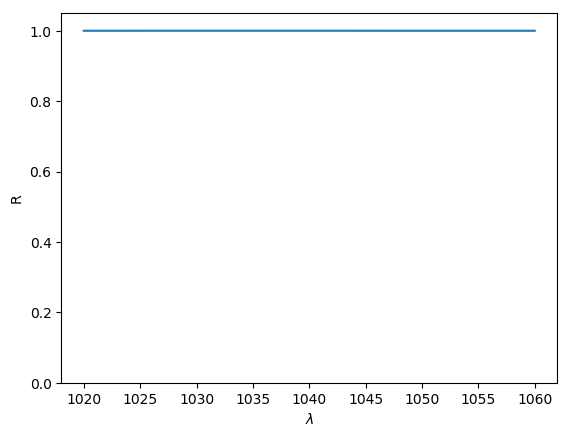
\includegraphics[width=\linewidth]{figures/wyniki/1stopien/opt10^5/result_Rresult10.png}
        \caption{R w iteracji 10}
    \end{subfigure}
        \begin{subfigure}[b]{0.31\textwidth}
        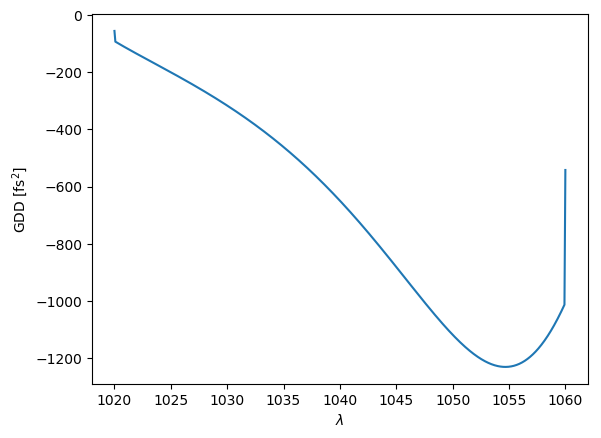
\includegraphics[width=\linewidth]{figures/wyniki/1stopien/opt10^5/result_gddresult10.png}
        \caption{GDD w iteracji 10}
    \end{subfigure}
        \begin{subfigure}[b]{0.32\textwidth}
        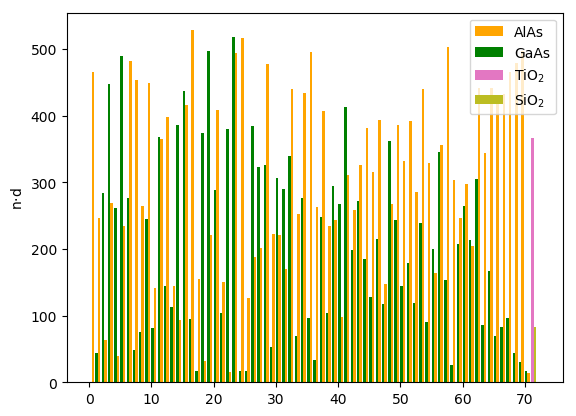
\includegraphics[width=\linewidth]{figures/wyniki/1stopien/opt10^5/result_ndresult10.png}
        \caption{Iloczyn $nd$ w iteracji 10}
    \end{subfigure}
    \caption{Wyniki obliczeń w przypadku losowania parametru wykorzystującego warunek Bragg'a przy wykorzystaniu współczynników załamania ze struktury 2}
    Wartości parametrów: $N= 100000$, $d_{near}= 0,005$, $w_{qual}=0,40$, $w_{best}=0,20$, $w_{better}=0,8$, $p_1=0,5$, $p_2=2$, $p_3=10$, $p_4=1$
    \label{fig:wyn1stpopt2}
\end{figure}

\subsection{Losowanie 2 parametrów korzystając z warunku Bragg'a i zależności między grubościami warstw} % df = n_warstw - n_warstw
Na koniec, inspirując się pracą \cite{dbr2}, gdzie z sukcesem udało się znaleźć dobre wyniki zarówno dla GDD i R korzystając z algorytmów genetycznych i prezentując dane w postaci dwóch parametrów: jeden zależny od warunku Bragg'a jak w przypadku poprzednim a drugi wprowadzający zależność między iloczynami $nd$ dla warstw w każdej parze, postanowiono sprawdzić czy również w przypadku algorytmów rojowych ta reprezentacja da rónie dobre wyniki. W tym celu zastosowano następujący układ równań:
\begin{equation}
    \left\{\begin{array}{l}
         n_1d_1 + n_2d_2 = \frac{\lambda_B}{2},  \\
         n_1d_1=h(n_1d_1 + n_2d_2) = h \cdot\frac{\lambda_B}{2}, \\
          n_2d_2=(1-h)(n_1d_1 + n_2d_2) = (1-h) \cdot\frac{\lambda_B}{2}, \\
          \lambda_B=\lambda\left[1+s\left(c-\frac 12\right)\right],
    \end{array}\right.
\end{equation}
gdzie: c, h --- zmienne przyjmujące wartości z zakresu $\langle0, 1\rangle$, które będą używane w algorytmie rojowym jako argument badanej funkcji (jedna para tych wartości odpowiada parze w strukturze DBR), s --- parametr pozwalający określić zakres wartości jakie przyjmuje $\lambda_B$. \\
Korzystając z tak przygotowanego układu równań, można wyznaczyć grubości warstw w danej parze:
\begin{equation}
    \left\{ \begin{array}{l}
         d_1 = \displaystyle\frac{h\lambda_B}{2n_1}, \\ d_2 = \displaystyle\frac{(1-h)\lambda_B}{2n_2}.
    \end{array}\right.
\end{equation}
Na podstawie tych wzorów sporządzono funkcję umożliwiającą transformację tablicy zmiennych $c$ i $h$ w tablicę grubości warstw w zwierciadle. Dodatkowo można było sporządzić funkcję odwrotną poprzez wyznaczenie wartości $c$ i $h$ zgodnie z:
\begin{equation}
    \left\{\begin{array}{l}
          c = \displaystyle\frac{2}{\lambda s}(n_1d_1 + n_2d_2) - \frac 1s + \frac 12, \\
           h = 1 + \displaystyle\frac{n_2d_2}{n_1d_1}.
    \end{array}\right.
\end{equation}

Na podstawie tak wyznaczonych zmiennych i funkcji dokonano obliczeń dla wielu zestawów parametrów funkcji celu. Najlepsze wyniki jakie udało się uzyskać przy użyciu współczynników załamania ze struktury 1 omawianej w \ref{sect:cel} przedstawiono na rysunku \ref{fig:wyn2stp1}, natomiast te przy użyciu współczynników załamania ze struktury 2 przedstawiono na rysunku \ref{fig:wyn2stp2}. Dodatkowo postanowiono sprawdzić, również tutaj, wpływ zmiany ilości zwiadowców na wynik. W tym celu przyjęto $N=100000$ i wykonano obliczenia, których rezultat został przedstawiony na rysunku \ref{fig:wyn2stp3}.

Można zauważyć, że wyniki przedstawione na rysunkach \ref{fig:wyn2stp1}, \ref{fig:wyn2stp2} i \ref{fig:wyn2stp3} są znacznie gorsze od wyników otrzymanych w poprzednich podejściach. Natomiast porównując je bezpośrednio do siebie, można zauważyć, że zmiana ilości par zwierciadeł DBR i wprowadzenie dodatkowych warstw z innych materiałów półprzewodnikowych znaczącą polepszyło rozwiązania na rysunku \ref{fig:wyn2stp2} względem \ref{fig:wyn2stp1}. Ponadto widać, że w tym wypadku, zwiększenie liczby pszczół zwiadowców nie wpłynęło szczególnie na jakość otrzymanego rozwiązania, natomiast zauważalnie przyspieszyło proces wyznaczenia rozwiązania finalnego, gdyż na rysunku \ref{fig:wyn2stp3} widać, że wykresy dla iteracji 0 jak i 10 są identyczne. Podsumowując, wyniki w przypadku algorytmu rojowego nie zyskują na jakości po wprowadzeniu tego sposobu reprezentacji danych, w odróżnieniu do algorytmów genetycznych. Możliwym sposobem na polepszenie wyników jest dopuszczenie zmiany ilości par zwierciadeł jak i dopuszczenie dodania dodatkowych warstw na koniec z innych materiałów. Takie rozwiązanie niestety nie zostało sprawdzone.

\begin{figure} [ht!]
    \centering
    \begin{subfigure}[b]{0.30\textwidth}
        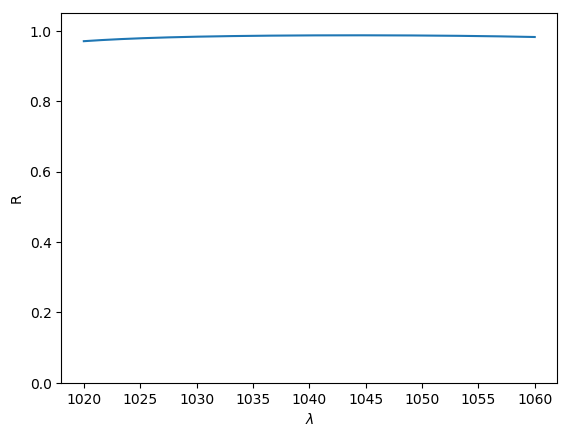
\includegraphics[width=\linewidth]{figures/wyniki/2stopien/dbr/result_Rresult0.png}
        \caption{R w iteracji 0}
    \end{subfigure}
            \begin{subfigure}[b]{0.31\textwidth}
        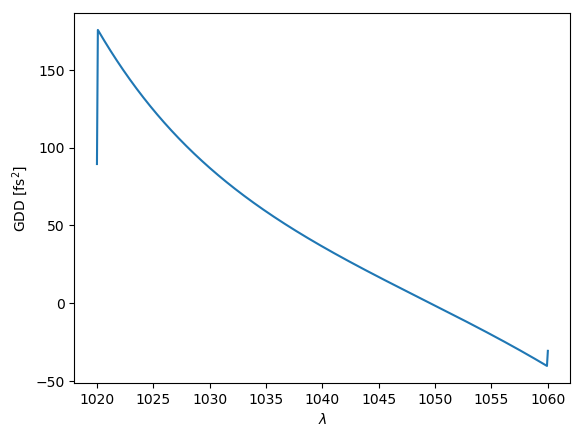
\includegraphics[width=\linewidth]{figures/wyniki/2stopien/dbr/result_gddresult0.png}
        \caption{GDD w iteracji 0}
    \end{subfigure}
        \begin{subfigure}[b]{0.32\textwidth}
        \includegraphics[width=\linewidth]{figures/wyniki/2stopien/dbr/result_ndresult0.png}
        \caption{Iloczyn $nd$ w iteracji 0}
    \end{subfigure}
        \begin{subfigure}[b]{0.30\textwidth}
        \includegraphics[width=\linewidth]{figures/wyniki/2stopien/dbr/result_Rresult499.png}
        \caption{R w iteracji 499}
    \end{subfigure}
        \begin{subfigure}[b]{0.31\textwidth}
        \includegraphics[width=\linewidth]{figures/wyniki/2stopien/dbr/result_gddresult499.png}
        \caption{GDD w iteracji 499}
    \end{subfigure}
        \begin{subfigure}[b]{0.32\textwidth}
        \includegraphics[width=\linewidth]{figures/wyniki/2stopien/dbr/result_ndresult499.png}
        \caption{Iloczyn $nd$ w iteracji 499}
    \end{subfigure}
    \caption{Wyniki obliczeń w przypadku losowania 2 parametrów przy wykorzystaniu współczynników załamania ze struktury 1}
    Wartości parametrów: $N= 1000$, $d_{near}= 0,05$, $w_{qual}=0,2$, $w_{best}=0,2$, $w_{better}=0,8$, $p_1=0.5$, $p_2=2$, $p_3=10$, $p_4=1$, $s=0.038$
    \label{fig:wyn2stp1}
\end{figure}

\begin{figure} [H]
    \centering
    \begin{subfigure}[b]{0.30\textwidth}
        \includegraphics[width=\linewidth]{figures/wyniki/2stopien/result_Rresult0.png}
        \caption{R w iteracji 0}
    \end{subfigure}
            \begin{subfigure}[b]{0.31\textwidth}
        \includegraphics[width=\linewidth]{figures/wyniki/2stopien/result_gddresult0.png}
        \caption{GDD w iteracji 0}
    \end{subfigure}
        \begin{subfigure}[b]{0.32\textwidth}
        \includegraphics[width=\linewidth]{figures/wyniki/2stopien/result_ndresult0.png}
        \caption{Iloczyn $nd$ w iteracji 0}
    \end{subfigure}
        \begin{subfigure}[b]{0.30\textwidth}
        \includegraphics[width=\linewidth]{figures/wyniki/2stopien/result_Rresult499.png}
        \caption{R w iteracji 499}
    \end{subfigure}
        \begin{subfigure}[b]{0.31\textwidth}
        \includegraphics[width=\linewidth]{figures/wyniki/2stopien/result_gddresult499.png}
        \caption{GDD w iteracji 499}
    \end{subfigure}
        \begin{subfigure}[b]{0.32\textwidth}
        \includegraphics[width=\linewidth]{figures/wyniki/2stopien/result_ndresult499.png}
        \caption{Iloczyn $nd$ w iteracji 499}
    \end{subfigure}
    \caption{Wyniki obliczeń w przypadku losowania 2 parametrów przy wykorzystaniu współczynników załamania ze struktury 2}
    Wartości parametrów: $N= 1000$, $d_{near}= 0,005$, $w_{qual}=0,4$, $w_{best}=0,2$, $w_{better}=0,8$, $p_1=10$, $p_2=20$, $p_3=10$, $p_4=5$, $s=0.038$
    \label{fig:wyn2stp2}
\end{figure}

\begin{figure} [H]
    \centering
    \begin{subfigure}[b]{0.30\textwidth}
        \includegraphics[width=\linewidth]{figures/wyniki/2stopien/morebees/result_Rresult0.png}
        \caption{R w iteracji 0}
    \end{subfigure}
            \begin{subfigure}[b]{0.31\textwidth}
        \includegraphics[width=\linewidth]{figures/wyniki/2stopien/morebees/result_gddresult0.png}
        \caption{GDD w iteracji 0}
    \end{subfigure}
        \begin{subfigure}[b]{0.32\textwidth}
        \includegraphics[width=\linewidth]{figures/wyniki/2stopien/morebees/result_ndresult0.png}
        \caption{Iloczyn $nd$ w iteracji 0}
    \end{subfigure}
        \begin{subfigure}[b]{0.30\textwidth}
        \includegraphics[width=\linewidth]{figures/wyniki/2stopien/morebees/result_Rresult10.png}
        \caption{R w iteracji 10}
    \end{subfigure}
        \begin{subfigure}[b]{0.31\textwidth}
        \includegraphics[width=\linewidth]{figures/wyniki/2stopien/morebees/result_gddresult10.png}
        \caption{GDD w iteracji 10}
    \end{subfigure}
        \begin{subfigure}[b]{0.32\textwidth}
        \includegraphics[width=\linewidth]{figures/wyniki/2stopien/morebees/result_ndresult10.png}
        \caption{Iloczyn $nd$ w iteracji 10}
    \end{subfigure}
    \caption{Wyniki obliczeń w przypadku losowania 2 parametrów przy wykorzystaniu współczynników załamania ze struktury 2}
    Wartości parametrów: $N= 100000$, $d_{near}= 0,005$, $w_{qual}=0,4$, $w_{best}=0,2$, $w_{better}=0,8$, $p_1=10$, $p_2=20$, $p_3=10$, $p_4=5$, $s=0.038$
    \label{fig:wyn2stp3}
\end{figure}

\section{Zastosowane technologie informatyczne}

Pod koniec tego rozdziału należy jeszcze odpowiedzieć na pytanie jakie technologie zostały wykorzystane przy pisaniu programu jak i przy samym liczeniu. 
Program został napisany w języku \textit{Python 3} z wykorzystaniem biblioteki \textit{numpy} do wykonywania obliczeń na macierzach oraz \textit{matplotplib} do wykonywania wykresów.

Cały algorytm podczas jednego cyklu wykonywał ok. miliona obliczeń trwających ok. $0,40\,$s każde, co skutkowało trudnością w uruchomienia go na komputerze osobistym ze względu na małą moc obliczeniową i co za tym idzie bardzo bardzo długim czasie wykonywania obliczeń (ponad 111 godzin). Dlatego też skorzystano z klastrów komputerowych pod nazwą \textit{Dragon} i \textit{Hydra} należących do Zespołu Fotoniki Instytutu Fizyki Politechniki Łódzkiej, co umożliwiło znaczne skrócenie obliczeń, do około 3 godzin przy wykorzystaniu 48 wątków na klastrze.

W celu wykorzystania dobrodziejstw klastra zastosowano bibliotekę \textit{mpi4py}, która pozwoliła na podział danych na poszczególne wątki i wykonywania obliczeń niezależnie. Później pod koniec każdej iteracji dane są zbierane do jednego wątku w celu podsumowania otrzymanych wyników.

Podsumowując udało się, z sukcesem, zastosować algorytmy rojowe w celu znalezienia zwierciadła DBR oferującego jak najmniejszą możliwą dyspersję opróżnienia grupowego. Niestety otrzymane wyniki są zauważalne gorsze od tych znajdujących się w literaturze (np. w \cite{dbr2}), lecz metoda ta pokazuje zauważalny potencjał. 